Sequential data and timeseries, causal relations, consequences of actions

Modelling temporal data is of fundamental interest in many branches of science.
This is understandable, since natural organisms inhabit a dynamic environment and
it is natural organisms, such as ourselves, that easily draw our attention and raise questions
deserving a scientific answer. The accuracy of the predictions, based on earlier observations,
is indeed a property that can easily affect the survival of the forecaster.  

Causality and consequences of actions are concepts tied to the passage of time.
Thus it is often time, that dictates the natural ordering of the datapoints
in sequential data. It is however not necessarily so, and any other single
physical dimension may also be used.

Commonly the sequential data is a result of making \emph{measurements} on a
\emph{system} of interest. In order to answer questions quantitatively,
the system and the measurements should be mathematically \emph{modelled}. The class of mathematical
models for dynamical systems we will be concerned with are called \emph{state space models} (SSMs).
Intuitively, SSMs make a clear distinction between the system itself and the measurements. At any instant,
the system is at a certain \emph{state}. In general, it is this state and its time evolution that we are interested in.
However the state is \emph{hidden} (or \emph{latent}) and the inference on the state has to be made entirely
based on the measurements.  Often some components of the measurements would otherwise translate directly to corresponding components of the state,
except that the measurements are always assumed to be \emph{noisy}. So even this part of the state is still latent.
To give a simple but often used example, consider the target tracking problem. In this case the state
could include the position and velocity of the target and our measurements could consists
of a sequence of noisy angular readings between the line of sight and a reference line. This situation is
known as \emph{bearings-only target tracking} \parencite{ristic2004beyond}.

The noisiness forces us to assume a probabilistic framework. In this thesis the viewpoint
is decidedly \emph{Bayesian}. In Bayesian statistics, ideally, the complete answer
is always the \emph{posterior probability distribution}, i.e. the joint probability distribution
of the random variables of interest given the measurements. Thus instead of answering
with a single value or a value with error bounds, the answer is the probability
density function of the interesting quantity given data. It is important to higlight,
however, that Bayesian statistics can be used to treat many kinds of uncertainty
\parencite{Sarkka2012a}. For example, the instruments used to obtain the measurements often incur
actual physical randomness modeled with Bayesian statistics, whereas the model parameters might in reality have some
exact ``true'' values, but our uncertainty about those values is still quantified with
Bayesian statistics. Thus applying statistical methods to a problem does not imply
that the problem is actually random.

SSMs are a general framework and in any specific situation prior knowledge of the
system has to be brought in. This prior knowledge is not necessarily very specific,
for example in ballistic target tracking it might include the assumption that Newton's
laws are applicable. The mathematical form of the dependence
between the measurements and the state has to be formulated as well as the dependence
of the state on its predecessors. Usually one is able only to specify the 
\emph{parametric} form for these equations. This results in a model with a set
of unknown parameters, denoted with $\Th$. Then, in order
to complete the model, these parameters need to be estimated based on some available
training data. This is sometimes, at least
in control engineering, known as \emph{system identification}. In this thesis,
it is assumed that the parameters are static, i.e. independent of time. 
This is then an important distinction between the states and
the parameters, in this thesis.

In general, assuming the aforementioned distinction between parameters and states, there are two separate but
interconnected estimation problems in SSMs: that of the states and that of the parameters. The interest might
lie in either one or both, depending on the model. Traditionally, state
estimation, given measurements up to the current instant, is known as \emph{filtering}.
The term can be thought to relate to the idea of filtering the noise out of the measurements
in order to observe the states. Given all the measurements, including the ones
\emph{after} the current time point, state estimation is called \emph{smoothing}.
Clearly, in order to do smoothing, one has to first collect all the measurements
and then go on with the estimation. Filtering, on the other hand, is an \emph{on-line}
procedure, i.e. the estimates can be updated every time a new measurement arrives.

A distinction is drawn in this thesis between \emph{linear} and \emph{nonlinear}
models. The linear model can be thought of as a special case of a nonlinear model,
so that the linear case would be implicitly covered by only considering nonlinear models.
The distinction is made for the simple reason that in the linear case, closed
form solutions exist. The Bayesian solution of the filtering problem for a linear system
with additive Gaussian noise is given by the celebrated \emph{Kalman filter} \parencite{Kalman1960}.

Our focus in this thesis is in the parameter estimation problem for the nonlinear case.
Depending on the method, this requires either the filtering or filtering and smoothing
solutions of the state estimation problem. For reasons of computational complexity, we will not however try to pursue
the the complete Bayesian solution of finding the posterior distribution. We will settle
for a point estimate called the \emph{maximum a posteriori} (MAP), which is the mode
of the posterior distribution. Under an assumed \emph{uniform} prior distribution,
the MAP estimate becomes equivalent with the \emph{maximum likelihood} (ML) estimate.
As will be seen, the distinction between these two, from the perspective of the
estimation equations, is not fundamental.

\begin{figure}[htb]%
    \centering%
    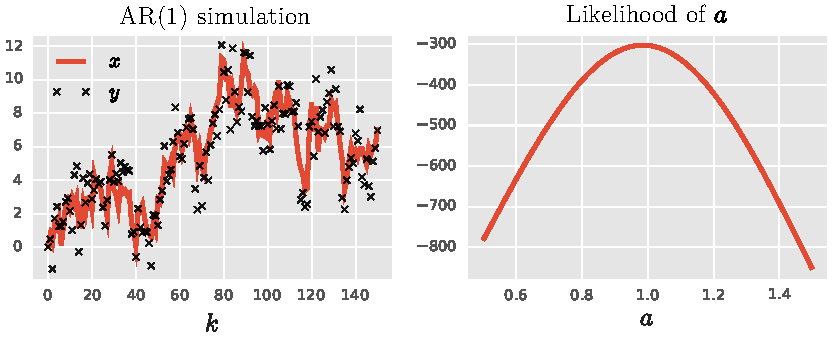
\includegraphics[width=\textwidth]{img/ar1_ex.pdf}%
	\caption{On the left: A simulation of the AR(1) model with $A=1$. The noisy measurements are denoted with crosses. On the right:
	A plot of the unnormalized probability distribution of $A$, given the simulated measurements and with a uniform prior.}
	\label{fig:ar1_simulation}
 \end{figure}

The structure of the thesis is as follows. We begin with the background, where
the SSMs are covered in necessary detail, the Bayesian optimal filtering
and smoothing equations are derived and the role of the static parameters is elaborated
on. Following the introduction we focus on on state estimation, first for linear
and then for nonlinear systems. The Kalman filter is introduced here as is the
concept of Gaussian filtering, a deterministic approximation used for nonlinear systems. 
The third chapter is concerned with the two methods
of parameter estimation we are comparing: gradient based nonlinear optimization
and the expectation maximization algorithm. The methods are analyzed in sufficient
theoretical detail in order to draw conclusions about the behavior of the methods
in the results section. The results section has three subsection: the analytical 
comparison of the competing algorithms from the point of view of convergence
and complexity, application with simulated data and an application with real world data.

State and measurement and modeling

Markov chain

Parameters, when and why are they interesting?

Bayesian approach, priors, probability distributions, uncertainty

Linear Gaussian 
  


Nonlinear Gaussian
  Bearings-only target tracking
  Stochastic volatility



